\subsubsection{MAC Adressen an Switchports}
\begin{figure}[!htb]
    \centering
    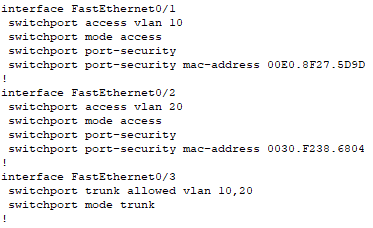
\includegraphics[width=.95\textwidth,height=.5\textwidth,keepaspectratio]{./img/config/mac-static/S1.png}
    \caption{Switch 1}
\end{figure}
\begin{figure}[!htb]
    \centering
    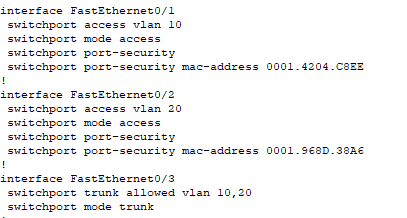
\includegraphics[width=.95\textwidth,height=.5\textwidth,keepaspectratio]{./img/config/mac-static/S2.png}
    \caption{Switch 2}
\end{figure}
\FloatBarrier
\subsubsection{Violation Modes}
Für die Tests wurde immer Fa0/2 auf Switch 1 konfiguriert. Die Security Adresse ist die default Adresse des Endsystems, welches zuvor eine neue MAC-Adresse zugewiesen bekommen hat, die jedoch nicht zurückgesetzt wurde zum testen.

\paragraph{Protect}
Bei Protect bemerkt man nichts außer, dass das System keine anderen Endsysteme erreichen kann und auch von anderen nicht erreicht werden kann, da es Netwerk nicht existiert. \\
\begin{figure}[!htb]
    \centering
    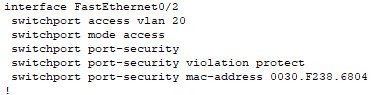
\includegraphics[width=.95\textwidth,keepaspectratio]{./img/config/security/protect/config.png}
    \caption{Switch 1 Fa0/2 Config}
\end{figure}
\begin{figure}[!htb]
    \centering
    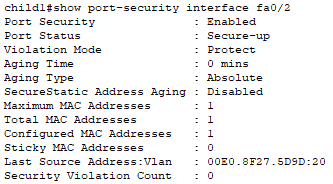
\includegraphics[width=.95\textwidth,height=.5\textwidth,keepaspectratio]{./img/config/security/protect/result.png}
    \caption{Resultat nach Ping}
\end{figure}
\FloatBarrier

\paragraph{Restrict}
Da die MAC-Adresse des Geräts nicht mit der am Port konfigurierten Adresse übereinstimmt, wird bei einem Ping-Versuch der Violation-Counter erhöht. Da Ping 4x einem echo sendet, wird der Counter um 4 erhöht. \\
\begin{figure}[!htb]
    \centering
    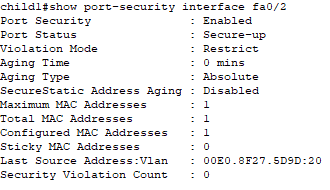
\includegraphics[width=.95\textwidth,keepaspectratio]{./img/config/security/restrict/Config.png}
    \caption{Switch 1 Fa0/2 Config}
\end{figure}
\begin{figure}[!htb]
    \centering
    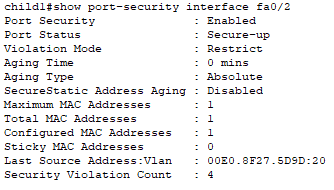
\includegraphics[width=.95\textwidth,height=.5\textwidth,keepaspectratio]{./img/config/security/restrict/Result.png}
    \caption{Resultat nach Ping}
\end{figure}
\FloatBarrier

\paragraph{Shutdown}
Da die MAC-Adresse des Geräts nicht mit der am Port konfigurierten Adresse übereinstimmt, ist die Verbindung bei einem Ping-Versuch ausgeschaltet worden.\\
\begin{figure}[!htb]
    \centering
    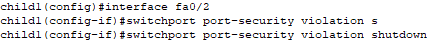
\includegraphics[width=.95\textwidth,keepaspectratio]{./img/config/security/shutdown/fa.png}
    \caption{Switch 1 Fa0/2 Config}
\end{figure}
\begin{figure}[!htb]
    \centering
    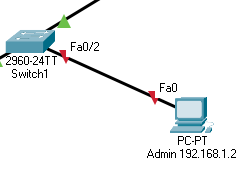
\includegraphics[width=.95\textwidth,height=.5\textwidth,keepaspectratio]{./img/config/security/shutdown/Result.png}
    \caption{Resultat nach Ping}
\end{figure}
\FloatBarrier

\subsubsection{Maximalwerte für die Anzahl an Adressen pro Port}
Um die Maximalwerte auprobieren zu können muss an dem Port ein Switch mit weiteren Geräten angehängt werden.Die Test fanden an Switch 1 Fa0/2 statt. Die max Anzahl ist 3.\\
\begin{figure}[!htb]
    \centering
    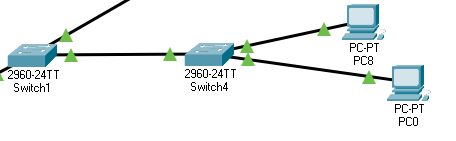
\includegraphics[width=.95\textwidth,height=.5\textwidth,keepaspectratio]{./img/config/max address/Protect_conf.png}
    \caption{Setup für die Test}
    Der 3.PC der zur Violation führt wurde immer aus- und eingehängt.
\end{figure}
\clearpage
\pagebreak
Abhängig vom Violation Mode wird die jeweilige Fehlerfunktion ausgeführt.
\vspace{5pt}
\\
\textbf{Protect:} Man bemerkt nur, dass man nicht senden kann. Aber als Admin bekommt man keine Violation Meldung.
\\
\textbf{Restrict:} Hier wird der Violation-Counter erhöht und die totalen Addressen bleiben beim Maximum. Man kann mehr Geräte einfügen, aber die Packets werden nicht weitergeleitet und der Counter wird für jedes Packet erhöht. Die registrierten Geräte können ganz normal Daten senden und erhalten ohne, dass der Counter erhöht wird.
\begin{figure}[!htb]
    \centering
    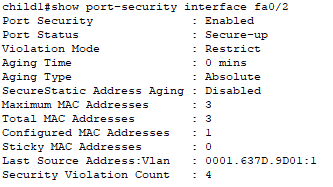
\includegraphics[width=.95\textwidth,keepaspectratio]{./img/config/max address/Protect.png}
    \caption{Switch 1 Fa0/2 nach Violation}
\end{figure}
\\
\textbf{Shutdown:} Sobald ein unbekanntes Gerät versucht was zu senden, geht das gesamte Port down und keiner kann was senden und erhalten.
\begin{figure}[!htb]
    \centering
    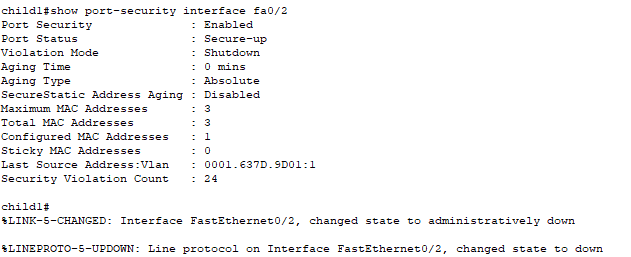
\includegraphics[width=.95\textwidth,keepaspectratio]{./img/config/max address/shutdown.png}
    \caption{Switch 1 Fa0/2 nach Shutdown}
\end{figure}
\FloatBarrier
\clearpage
\pagebreak
\subsubsection{Frage 3}
\paragraph{Frage}
Wie unterscheiden sich die Violation-Modes (Vor-/Nachteile), wie
ändern sich die Source Address Tables der Switches durch die unterschiedlichen
Konfigurationen, und wie kann Port Security umgangen werden?
\paragraph{Antwort}
\textbf{Violation Modes}
\begin{table}[!htb]
    \centering
    \begin{tabular}{ |m{3.7em}|m{13.2em}|m{13.1em}| }
        \hline
        \thead{Mode} & \thead{Vorteile}                                                                                                                                         & \thead{Nachteile}                                                                                                                       \\
        \hline
        protect      & Das System bleibt immer aktiv. Ist gut geeignet für Netze, wo man einfach nur die Menge an parallen Verbindungen reduzieren will.                        & Gegen Angriffe nicht wirklich geschützt. Nicht für Netzwerke die sensible Daten übertragen sollen geeignet.                             \\
        \hline
        restrict     & Ist gut geeignet für Gruppierungen und wenn das Netz bei Angriffen bzw. Violations nicht gleich abgedreht werden muss, aber man das Netz Monitoren will. & Wie "protect" nicht wirklich gegen Angriffe geschützt. Nicht für Netzwerke die sensible Daten übertragen sollen geeignet.               \\
        \hline
        shutdown     & Für spezielle Fälle geeignet, wo nur ganz bestimmte Geräte in der Lage sein sollten sich zu verbinden.                                                   & Für Weitervernetzung nicht wirklich geeignet, da dann alle Systeme am Port gleich getrennt werden, sollte es zu einer Violation kommen. \\
        \hline
    \end{tabular}
\end{table}
\\
\textbf{SATs der Switches}\\
Adressen an den Ports nach der Konfiguration einer statischen MAC-Adresse, werden als statisch in der SAT gespeichert. Bis auf die Switch Adressen werden alle anderen nach der aging time gelöscht.
\vspace{5pt}\\
\textbf{Wege zum umgehen der Port Security}
\\
Wenn man die MAC-Adresse des konfigurierten Ports kennt, kann man MAC spoofing anwenden und sich einfach einbinden.
Eine weitere Problematik kann sich ergeben, wenn jemand versucht durch "Brute Forcing" einzudringen und die Port Security zb. nicht auf Shutdown eingestellt ist.